\documentclass[journal,10pt]{IEEEtran}
\usepackage{amsmath,amssymb,graphicx,booktabs,array,cite,url}
\newtheorem{proposition}{Proposition}
\newcommand{\ind}{\mathbb{I}}
\newcommand{\uj}{\,\mu\mathrm{J}}
\newcommand{\us}{\,\mu\mathrm{s}}
\setlength{\tabcolsep}{4pt}
\hyphenation{acknowledgement acknowledgements datagram datagrams}
\begin{document}
\title{Energy-Feasible Fragment Recovery for Clustered IoT Networks: Fixed-Window Accounting and Shared-Head Evaluation}
% Insert verified author names, affiliations and corresponding-author details here.
\author{}
\maketitle
\begin{abstract}
Energy-harvesting Internet of Things networks must complete packet transfers with energy that is available at both the source and its forwarding head. Fragment recovery can reduce retransmission cost, but its benefit depends on acknowledgement overhead, retained receiver state, finite buffers, and the energy spent while a source waits for forwarding confirmation. This paper presents a deterministic, energy-feasible fragment-recovery framework with explicit control costs and fixed-duration transaction settlement. The framework combines source-specific fragment identities, cumulative acknowledgement bitmaps, jointly funded transmission windows, deadline-aware service, and receipt-based custody release. A shared-head extension accounts for competing sources, a common relay battery, a bounded reassembly buffer, and serialized frame airtime. Three controlled studies comprise 64,512 simulated episodes over 160 distinct paired development seeds. In the shared-head study, selective recovery with block acknowledgements achieves 17.12\% timely delivery and 57.87 delivered packets per charged joule, compared with 12.56\% and 41.45 for whole-packet retry and 13.49\% and 44.58 for per-fragment selective retry. All four family-adjusted lower confidence bounds exceed the prespecified 1\% improvement margin. Affordable-prefix and last-frame completion variants do not improve on the block-acknowledgement comparator. The results identify feedback amortization and consistent transaction accounting as useful design choices, while exposing the delivery limits imposed by concentrated relay resources in the evaluated IoT setting.
\end{abstract}
\begin{IEEEkeywords}
Internet of Things, energy harvesting, medium access control, fragment recovery, block acknowledgement, energy causality, deadline-aware communication.
\end{IEEEkeywords}

\section{Introduction}
\IEEEPARstart{E}{nergy}-harvesting IoT devices support sensing where battery replacement is costly. Yet replenishment does not guarantee communication: a source may afford transmission while its forwarding head cannot afford reception and forwarding. Conversely, a funded head cannot recover data discarded before confirmation. MAC design must coordinate energy, packet state, and each participant's received information.

Energy-aware access has long been studied as a problem distinct from conventional battery-lifetime maximization~\cite{iannello}. A further issue arises when an application datagram occupies several link-layer frames. Fragmentation is an established part of constrained-IP communication~\cite{rfc4944}. A single missing fragment can prevent application delivery despite successful reception of most of the datagram. Repeating the entire datagram wastes successful work, whereas retaining partial reception introduces buffer occupancy, acknowledgement state, and recovery decisions. Standards already provide fragment forwarding and selective recovery mechanisms~\cite{rfc8930,rfc8931}; their existence motivates a careful accounting question rather than another claim that selective retransmission is new.

Acknowledgements consume energy and determine received knowledge. A head or sink may receive data without its sender learning that fact. Releasing source custody after hidden sink completion leaks information; shortening listening after an unobserved forwarding failure understates energy. Either error can change policy rankings.

We reserve each transaction's member, forwarding, and feedback costs from current source and head batteries. A fixed receipt boundary preserves charged listening even when forwarding positions are unused. Decisions use paid reports and received acknowledgement state, never future harvest or hidden delivery knowledge.

We compare whole-packet retry, per-fragment selective retry, and selective recovery with block feedback. Two additional variants test affordable-prefix admission and a final-frame completion guard. Shared-head integration introduces competition for the same head energy and buffers. Unsuccessful variants remain part of the reported evidence.

Our contributions are a local-information model separating delivery from custody release; joint energy, queue, reassembly, and airtime constraints with safety properties; and paired evidence, negative variants, and resource sensitivity across 64,512 episodes. The contribution is their integration and evaluation: block acknowledgements and selective recovery are established prior art.

\section{Related Work and Study Position}
\subsection{Energy-Aware Access and Receiver Coordination}
Iannello \emph{et al.}~\cite{iannello} analyze access with replenishable energy. We address the narrower interaction of fragment progress, received knowledge, and joint two-hop funding.

Receiver coordination is also an established source of energy savings. RI-MAC~\cite{rimac} uses receiver-initiated exchanges to support asynchronous duty cycling and dynamic traffic. TSCH describes scheduled channel access for low-power communication~\cite{rfc7554}, while the minimal 6TiSCH configuration specifies an interoperable operating baseline~\cite{rfc8180}. These mechanisms show why listening and control exchanges should be included in an energy comparison. Our transaction schedule uses serialized windows but does not implement a TSCH or 6TiSCH stack.

Recent adaptive-listening and energy-aware scheduling studies optimize receiver wake times, slotframes, or routes. Table~\ref{tab:related} gives their reported operating points and evidence types. Our complementary question is how an already scheduled link completes fragmented messages under joint energy and custody constraints. RL-ASL's hardware validation and the battery-less 6TiSCH study's full-stack evaluation exceed the deployment scope of our component simulator. Their numerical results are context, not a common leaderboard.

\subsection{Fragment Forwarding and Recovery}
RFC~4944~\cite{rfc4944} establishes fragmentation for IPv6 over IEEE~802.15.4. RFC~8930~\cite{rfc8930} addresses forwarding fragments over multiple hops, and RFC~8931~\cite{rfc8931} adds selective recovery with acknowledgement bitmaps and congestion-control support. These specifications establish both the mechanism family and the need to manage outstanding fragments. Our custom format uses six fragments and compact identities to expose the relevant costs; it is not an implementation-conformance study of those RFCs.

The distinction between retained physical progress and received knowledge is central here. Decisions use the bitmap that arrived, not the bitmap that was transmitted, at both hops and at final custody release.

\subsection{Relationship to Cluster-Head Selection}
The HEART-CH manuscript~\cite{heart} describes hybrid-energy, spatiotemporal control of cluster-head identities. Its controller and the MAC layer address different decisions: selecting a head determines the forwarding role, while fragment service determines which queued data can complete through the assigned role. The present experiments hold head identities exogenous and model either a fixed head or one prescribed change. They therefore isolate MAC behavior without attributing clustering or mobility benefits to fragment recovery.

Table~\ref{tab:related} summarizes the scope. Numerical comparisons use local implementations with common physical accounting, stochastic inputs, and deadlines; literature comparisons establish mechanism context.

\begin{table*}[t]
\caption{Recent literature: reported results and comparison boundaries (different workloads and energy denominators)}
\label{tab:related}\centering\small
\begin{tabular}{p{.18\textwidth}p{.39\textwidth}p{.34\textwidth}}
\toprule Work & Reported evidence and operating point & Distinction from this study \\
\midrule
PRIL-ML~\cite{scanzio}, 2024 preprint & Analytical estimate at $r=4$: 83.8~$\mu$W and 9.231~s latency; simulated PRIL-M: 68.6~$\mu$W and 30.58~s slow-flow latency. & Sleep/latency tradeoff. Our fragment component is executed in simulation; this does not imply lower power or delay.\\
Battery-less 6TiSCH~\cite{vanleemput}, 2024 & Cooja plus harvesting model; 21 nodes, ten 9-hour runs per condition. Reporting 90.19\%, uptime 91.10\%, latency 627~ms (32.28\% increase). & Energy-aware scheduling/routing with broader stack and harvest coverage; recovery semantics and endpoints differ.\\
RL-ASL~\cite{rlasl}, 2026 preprint & FIT IoT-LAB hardware: simple-topology mean power 0.561 versus 0.996~mW for Orchestra; star: 0.647 versus 1.008~mW. & Receive-slot activation with stronger physical validation. No matched energy or reliability ranking against our model.\\
HEART-CH~\cite{heart}, supplied manuscript & Cluster-head selection; 20 episodes per comparison; reconstructed Welch tests for component ablation. & Upstream role selection. We retain paired seeds and isolate fragment service with prescribed heads.\\
This work & Shared-head simulation: 32 paired seeds; 17.121\% timely delivery and 57.8723 packets/J; 36.34\% and 39.61\% gains over matched whole retry. & Joint funding, feedback-local knowledge, finite custody and exact ledgers; advantage is established only over local matched baselines.\\
\bottomrule
\end{tabular}
\end{table*}

\section{System Model}
\subsection{Nodes, Packets, and Frame Order}
Consider $M$ IoT sources, two possible forwarding heads, and a gateway. Only one head serves the sources in a frame. Time is divided into $H=24$ frames of duration $T_f=1$~s, indexed by $t=0,\ldots,H-1$. The prescribed head is denoted by $h(t)$. A change, when enabled, occurs at $t=12$. The inactive head still incurs the background energy cost while alive. Heads do not generate application traffic in these component experiments.

Source $i$ generates at most one datagram per frame, with
\begin{equation}
A_i(t)\sim\operatorname{Bernoulli}(p_a),\qquad p_a=0.35.
\label{eq:arrival}
\end{equation}
A packet identity is the pair $p=(i,b)$, where $b$ is its birth frame. Its deadline is $d_p=b+\tau$, with $\tau\in\{2,6\}$. Successful forwarding must complete strictly before $d_pT_f$. Source queues retain at most two datagrams, including delivered datagrams whose final receipt has not arrived. A new arrival to a full queue is an overflow loss. A packet generated after source death is recorded as a death loss, so offered traffic does not disappear from the denominator.

Within each frame, the simulator applies background expenditure, expires old state, generates arrivals, performs funded controls, executes admitted transactions, and finally adds harvest to surviving nodes. This order matters: newly harvested energy becomes available only after the current frame's communication. A packet that reaches its deadline is expired before that frame's admission decisions.

\begin{figure*}[t]
\centering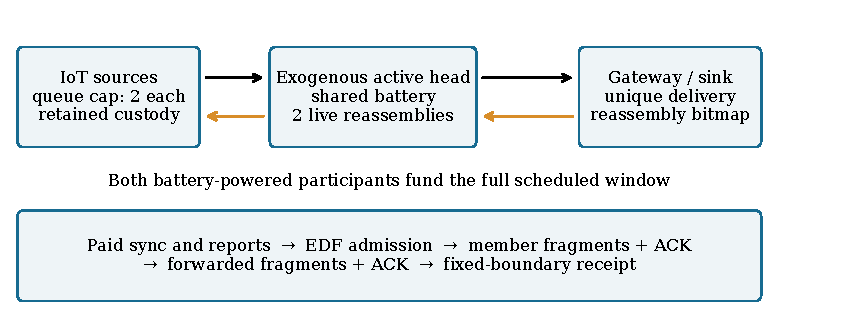
\includegraphics[width=.94\textwidth]{figures/architecture.pdf}
\caption{Evaluated two-hop IoT data path and transaction order. Forward arrows carry fragments; reverse arrows carry received acknowledgement state. All sources share the active head's energy and two live reassembly buffers. Head identities are externally prescribed.}
\label{fig:architecture}
\end{figure*}

\begin{table}[t]
\caption{Principal notation}\label{tab:notation}\centering\small
\begin{tabular}{p{.22\columnwidth}p{.69\columnwidth}}\toprule
Symbol & Meaning\\\midrule
$M,H,T_f$ & Source count, horizon, and frame duration\\
$p=(i,b),d_p$ & Source-specific packet identity and deadline\\
$Q_i(t)$ & Source custody queue\\
$B_n,C_n$ & Current energy and battery capacity of node $n$\\
$a_n(t)$ & Alive indicator\\
$F_n(t)$ & Energy available after protecting future sleep\\
$C_{h,p}$ & Fragments physically cached at head $h$\\
$\widehat C_{i,p}$ & Head bitmap last received by source $i$\\
$S_p,\widehat S_{h,p}$ & Sink bitmap and head's received sink bitmap\\
$\mathcal U_p,\mathcal V_p$ & Planned member and forwarding fragment sets\\
$W_p$ & Fixed duration of one granted transaction\\
$D,G,E$ & Unique timely deliveries, generated packets, charged energy\\
\bottomrule\end{tabular}
\end{table}

\subsection{Energy Causality and Absorbing Death}
All battery values and debits are represented as integer microjoules. At each frame start, an alive node pays up to $e_0=60\uj$ for its background operation. Reaching zero energy causes absorbing death. The current spendable credit, evaluated after this debit and updated after each control or transaction, is
\begin{equation}
F_n(t)=a_n(t)\max\{0,B_n- e_0(H-t-1)\}.
\label{eq:credit}
\end{equation}
This reserve protects the remaining background costs over the declared horizon. It does not reserve future control traffic or assume that future harvest will occur. The reserve is a common scheduling constraint, not a prediction of the harvesting process.

Let $c_n(t)$ be the total actual debit in frame $t$, and let $B_n^+(t)$ denote energy after that debit. Then
\begin{align}
B_n^+(t)&=B_n(t)-c_n(t)\geq0,\\
g_n(t)&=a_n^+(t)\min\{h_n,C_n-B_n^+(t)\},\\
B_n(t+1)&=B_n^+(t)+g_n(t).
\label{eq:battery}
\end{align}
Here $h_n$ is the constant offered harvest in a scenario and $a_n^+(t)$ is zero after death. A dead node is not revived by later harvest. This battery-backed lifecycle differs from intermittent devices designed to reboot after energy recovery. Each policy uses the same lifecycle and capacity within a paired scenario.

\subsection{Fragment and Feedback State}
Every datagram contains 500 payload bytes, divided into
\begin{equation}
(\ell_0,\ldots,\ell_5)=(99,99,99,99,99,5).
\end{equation}
The complete fragment set is $\mathcal F=\{0,\ldots,5\}$, represented by the six-bit mask $63$. Each fragment includes an eight-byte header with birth identifier, source identity, fragment index, and count. A 26-byte physical/MAC/security allowance gives a maximum on-air length of 133 bytes, including six physical-layer bytes. The allowance is an accounting choice, not a security evaluation.

The model distinguishes four states: the head's physical cache $C_{h,p}$, the source's last received head bitmap $\widehat C_{i,p}$, the sink's physical bitmap $S_p$, and the head's last received sink bitmap $\widehat S_{h,p}$. For persistent recovery, successful fragment reception applies set union. Knowledge is updated only when its corresponding acknowledgement arrives. Neither the source nor head receives the simulator's unique-delivery set as an observation.

The source releases a packet only after a complete final receipt. The head may release its payload cache after receiving a complete sink acknowledgement, even if the source has not received the relayed receipt. A small confirmation record supports later receipt recovery. In the shared-head model, all such metadata expires at the packet deadline. The earlier single-source engine permits confirmation records to persist until head death or the finite horizon; these records are not additional live payload buffers.

\subsection{Channel Outcomes and Head Changes}
The single-source studies include clean data delivery, independent fragment success probability $0.9$, and a burst model with a common success event for a hop and frame. In the shared-head study, the burst event is keyed by source, hop, and frame; fragments of that source on that hop share the event. This is not a spatially common interference model. Data success and acknowledgement reception are separately sampled. ACK and final-receipt erasure probability is zero or $0.1$ in the single-source grid and $0.1$ in the shared grid.

Sync, reports, and grants are assumed reliable when funded. This assumption isolates data/feedback recovery and bounds the interpretation of the results. All required control transmission and listening costs are nevertheless charged. On paid discovery of a different head, a source clears its old head-knowledge bitmap. Physical fragments at an old head are not transferred for free. Sink reassembly can persist until expiry, but the new head must obtain its own acknowledgement state through the modeled exchange.

\section{Energy-Feasible Fragment-Recovery Method}
\subsection{Wire Time and Fixed Radio Windows}
The radio model uses a 250-kbit/s rate informed by the CC2420 specifications~\cite{cc2420}. With two $400\us$ guards and a $192\us$ turnaround/gap allowance, the duration of a modeled frame containing $L$ on-air bytes is
\begin{equation}
T(L)=800+32L+192\quad[\mu\mathrm{s}].
\label{eq:wire}
\end{equation}
Define $T_k=T(8+\ell_k+26)$ for data fragment $k$, $T_A=T(9+26)$ for a cumulative ACK, and $T_G=T(14+26)$ for a grant. These give $T_A=2112\us$ and $T_G=2272\us$. The nine-byte ACK identifies the packet, source, head, and bitmap. The grant communicates the head epoch, identities, and selected fragment masks.

For planned member set $\mathcal U_p$ and forwarding set $\mathcal V_p$, the reserved transaction duration is
\begin{equation}
W_p=T_G+\sum_{k\in\mathcal U_p}T_k+
\sum_{k\in\mathcal V_p}T_k+(n_A+1)T_A.
\label{eq:window}
\end{equation}
The extra ACK interval is the final receipt. Per-fragment selective retry uses $n_A=|\mathcal U_p|+|\mathcal V_p|$; block feedback uses
\begin{equation}
n_A=\ind[|\mathcal U_p|>0]+\ind[|\mathcal V_p|>0].
\end{equation}
Both participants remain charged through $W_p$, including unused forward positions and lost feedback. Actual forwarding is restricted to available cached fragments. The final receipt is placed at the end of the reserved window, so its timing does not reveal hidden channel outcomes to the source.

The active increment above the background floor is $P_\Delta=0.05634\uj/\us$. This represents a conservative receive-power envelope for both battery-powered participants, with role-dependent processing allowances:
\begin{align}
e_{i,p}&=\lceil P_\Delta W_p\rceil+2\uj,\\
e_{h,p}&=\lceil P_\Delta W_p\rceil+22\uj.
\label{eq:cost}
\end{align}
At 3~V the typical receive current of 18.8~mA corresponds to 56.4~mW~\cite{cc2420}; the model separates its 60-$\mu$W floor from the active increment. These are device-informed simulation costs. They do not include a measured firmware implementation, gateway energy, or an optimized schedule of radio power transitions.

\subsection{Paid Observation and Joint Admission}
In the shared-head experiment, one paid broadcast synchronization interval precedes individually serialized source reports. Its duration is $1192+T(33)\us$. A report contains current source credit, at most two birth/deadline pairs, and two received head bitmaps. The 31-byte report incurs $T(31+26)\us$. Each participating source pays for synchronization and its own report; the head pays for the synchronization and every received report. A ten-microjoule allowance is included for each such control operation in the shared engine. The single-source engine instead applies one ten-microjoule allowance to its combined control window, as specified in its frozen configuration.

Admitted packets are ordered by earliest deadline. The shared-head tie order rotates source priority with the frame index. Reported credit is reduced by public, deterministic transaction debits when a source receives more than one grant. The head uses current local energy and reassembly state. For a packet to be admitted, its proposed window must satisfy
\begin{align}
e_{i,p}&\leq F_i(t),&e_{h,p}&\leq F_h(t),\label{eq:funding}\\
u+W_p&\leq T_f,&n_i&<2,\label{eq:airtime}\\
n_{\mathrm{all}}&<24,&|\mathcal B_h|&\leq2,\label{eq:caps}
\end{align}
where $u$ is elapsed frame airtime, $n_i$ and $n_{\mathrm{all}}$ count granted packets, and $\mathcal B_h$ contains live head reassemblies. A new identity is refused when both head payload buffers are occupied. The implementation also conservatively applies that check to a new confirmation-only identity. Cached identities can continue without consuming another payload slot.

Equation~\eqref{eq:airtime} checks wire duration as well as packet count. Nonparticipating sources pay background cost. The announced timing is assumed to be followed within the fixed guard allowance.

\subsection{Compared Recovery Policies}
\emph{Whole-packet retry} reserves six member and six forwarding fragments for each attempt. If the head has not received the full datagram in that attempt, forwarding is suppressed while the prepaid window remains charged. Partial receiver progress is reset at the next attempt. Its feedback is block-based, so the comparison does not artificially penalize it with per-fragment ACKs.

\emph{Per-fragment selective retry} preserves received fragments and sends a cumulative ACK after each transmitted fragment. Initially, its planned sets are
\begin{align}
\mathcal U_p&=\mathcal F\setminus\widehat C_{i,p},\\
\mathcal V_p&=(C_{h,p}\cup\mathcal U_p)\setminus\widehat S_{h,p}.
\label{eq:sets}
\end{align}
If the resulting window is unaffordable, the rule removes trailing new member fragments and recomputes forwarding. Once member fragments are exhausted, it reduces forwarding. Thus, the selective comparator can exploit affordable partial windows rather than being forced to wait for full funding.

\emph{Block acknowledgement} uses the same persistent fragment state and initial sets~\eqref{eq:sets}, but one cumulative ACK per nonempty hop block. It admits the full planned missing-fragment window when jointly affordable. If neither hop needs data and the head has complete sink confirmation, a grant-plus-receipt transaction can release source custody.

\emph{Affordable block prefix} applies the selective comparator's truncation order to block feedback. This rule tests whether using residual energy for partial progress improves over waiting for a complete planned block. It is a separate candidate, not a change to the block comparator after observing outcomes.

\emph{Last-frame completion guard} further declines a prefix transaction in the final usable frame unless the head's local cache, planned member fragments, and received sink bitmap jointly cover the complete packet, and the planned forwarding plus received sink bitmap cover completion. Lost feedback can make the rule conservative: actual sink completion need not be known at the head. The guard is therefore an observable-state heuristic rather than a guarantee of successful completion.

\begin{figure}[t]
\hrule\vspace{4pt}
\textbf{Algorithm 1: Funded shared-head fragment service}
\begin{enumerate}\setlength\itemsep{1pt}
\item Pay background cost; apply absorbing death; expire packet state.
\item Generate source arrivals and enforce the two-packet custody queues.
\item Fund the active head's synchronization and eligible source reports.
\item Decode reports; reset source head knowledge on an observed change.
\item Order reported packets by deadline and rotating source tie priority.
\item For each eligible packet, construct the policy's fragment sets.
\item Check joint energy, shared buffer, packet budget, and frame duration.
\item Issue the paid grant and execute member fragments with policy feedback.
\item Forward only available fragments; update local state on received ACKs.
\item Keep both participants funded until the fixed final-receipt boundary.
\item Release source custody only on a received complete receipt; settle debits.
\item Add harvest to surviving nodes and verify packet/energy conservation.
\end{enumerate}
\vspace{2pt}\hrule
\caption{Deterministic service order. Decisions use current paid reports and local state; the channel tape and global delivery ledger are environment-only variables.}
\label{fig:algorithm}
\end{figure}

\section{Accounting Properties and Complexity}
\subsection{Energy and Packet Conservation}
The following properties concern the specified execution model. They establish feasibility and accounting consistency, not an optimality claim for EDF or any recovery policy.

\begin{proposition}
If each admitted transaction satisfies~\eqref{eq:funding}, its fixed-window settlement cannot overdraw either participating battery.
\end{proposition}
\begin{IEEEproof}
Equation~\eqref{eq:credit} gives $0\leq F_n(t)\leq B_n$. Admission bounds the scheduled debit by $F_n(t)$, and settlement charges exactly that debit, independently of fragment or ACK outcomes. Subtraction therefore preserves nonnegative battery energy. The same argument applies sequentially because subsequent admissions use updated credit. Background costs are capped by current battery energy and harvest is added only afterward.
\end{IEEEproof}

For every battery-powered node, the implementation checks
\begin{equation}
B_n(0)+\sum_t g_n(t)=B_n(H)+\sum_t c_n(t).
\label{eq:energyledger}
\end{equation}
Harvest that would exceed capacity is not included in $g_n(t)$. The network debit is decomposed into background, control, member-data, forwarding-data, and feedback/padding categories. Rounding and processing residuals are assigned to the last category, so their sum equals actual integer debits. The partition is useful for diagnosis, although feedback/padding is broader than the energy of ACK bytes alone.

\begin{proposition}
Unique timely delivery and receipt-based custody can coexist without double-counting a datagram or removing an unconfirmed source copy.
\end{proposition}
\begin{IEEEproof}
The sink credits an identity only once, after its complete bitmap is available before the deadline. Subsequent copies do not add another delivery. Source deletion requires a received complete final receipt and is evaluated separately. A lost receipt therefore retains source custody without changing the unique-delivery count. Source-specific identity validation prevents a fragment of one source from satisfying another source's packet.
\end{IEEEproof}

Let $G$ denote generated datagrams, $D$ unique timely deliveries, and $L_{\mathrm{exp}}$, $L_{\mathrm{ov}}$, $L_{\mathrm{dead}}$, and $P$ the expired, overflow, death, and pending-undelivered counts. The terminal partition satisfies
\begin{equation}
G=D+L_{\mathrm{exp}}+L_{\mathrm{ov}}+L_{\mathrm{dead}}+P.
\label{eq:packetledger}
\end{equation}
A delivered packet retained for receipt recovery belongs to $D$, not to $P$. This distinction prevents feedback loss from turning an already credited delivery into an artificial pending or expired loss.

\subsection{What Block Feedback Saves}
For a fixed pair of fragment sets with sizes $m$ and $f$, the difference between per-fragment and block-feedback reservations is
\begin{equation}
\Delta W=\{m+f-\ind[m>0]-\ind[f>0]\}T_A.
\label{eq:saving}
\end{equation}
For $m=f=6$, block feedback eliminates ten ACK intervals, saving $21120\us$ of reservation. Under the common radio envelope, the two participants' active-energy reduction is approximately $2P_\Delta\Delta W=2379.8\uj$, before integer rounding. This is a same-action accounting identity. Across a rollout, the policies may admit different transactions and preserve different knowledge, so~\eqref{eq:saving} is not a proof of end-to-end dominance.

Persistent recovery also changes the value of partial data reception. Under independent fragment success probability $q$, a complete six-fragment hop in one attempt has probability $q^6$. For two complete independent hops, the corresponding data-only event has probability $q^{12}$. At $q=0.9$, this is approximately $0.2824$, before feedback and energy constraints. Retaining fragments avoids requiring all successes to coincide in one attempt, but consumes finite state across attempts. This elementary comparison helps explain why the benefit of persistence depends on the erasure correlation model.

\subsection{Computational and Storage Cost}
With two reported datagrams per source, EDF ordering operates on at most $2M$ entries and costs $O(M\log M)$. For $F$ fragments, set construction and the bounded truncation rule require at most $O(F^2)$ work in a direct implementation. Here $F=6$, so these operations have small fixed bounds. Processing at most two grants per source gives a per-frame upper bound of $O(M\log M+MF^2)$ before applying the global 24-grant and airtime limits.

Payload storage is bounded by two datagrams per source and two live datagrams per head. Fragment bitmaps require $F$ bits per tracked identity, in addition to identity and deadline metadata. The sink's unique-delivery bookkeeping is an evaluation function and is not counted as constrained-device memory. These bounds characterize the implemented state organization; no processor execution time or embedded RAM measurement is inferred from the Python experiment runtime.

\section{Experimental Protocol}
\subsection{Study Grids and Paired Inputs}
Table~\ref{tab:setup} lists the two physical grids. The corrected single-source study evaluates four policies on 64 paired seeds, giving $96\times64\times4=24576$ episodes. A separate 64-seed study evaluates the completion guard and four comparators, giving 30720 episodes. The shared-head study evaluates three policies on 32 new paired seeds, giving 9216 episodes. The valid corpus therefore contains 64512 episodes and 160 distinct seed units.

The single-source studies use seeds 9700100--9700163 and 9700200--9700263; the shared-head study uses 9710000--9710031. Seeds within each study are independent simulation units. Scenarios and policies within a seed share exogenous inputs. Arrival, data, acknowledgement, receipt, and burst values are indexed by physical event identity rather than consumed according to policy actions. This avoids changing the channel realization merely because one policy makes fewer transmissions.

All policy definitions, scenario grids, endpoints, and decision margins were fixed before each study's performance execution. An earlier variable-window implementation was excluded after an accounting audit found that hidden forwarding outcomes could shorten charged waiting time. Its performance estimates are not used here. The corrected model reserves the complete window and places the final receipt at a fixed boundary. This change addresses measurement validity rather than selecting a favorable result from the excluded run.

\begin{table}[t]
\caption{Simulation configuration}\label{tab:setup}\centering\small
\begin{tabular}{p{.35\columnwidth}p{.25\columnwidth}p{.27\columnwidth}}\toprule
Parameter & Single source & Shared head\\\midrule
Sources $M$ & 1 & 1, 4, 12\\
Possible heads & 2 & 2\\
Horizon / frame & 24 / 1 s & 24 / 1 s\\
Capacity (mJ/node) & 4, 16 & 16, 64\\
Harvest ($\mu$J/frame) & 0, 300 & 0, 1200\\
Deadline (frames) & 2, 6 & 2, 6\\
Arrival probability & 0.35 & 0.35\\
Head schedule & Fixed, switch & Fixed, switch\\
Data law & Clean, iid, burst & iid, burst\\
Lossy data success & 0.9 & 0.9\\
ACK erasure & 0, 0.1 & 0.1\\
Source queue cap & 2 & 2 per source\\
Head payload cap & 2 & 2 total/head\\
Global grant cap & 2 & 24\\
Per-source grant cap & 2 & 2\\
Scenario cells & 96 & 96\\
CPU workers & 8 & 8\\\bottomrule
\end{tabular}
\end{table}

\subsection{Endpoints and Uncertainty}
For policy $\pi$, seed $s$, and scenario $k$, let $D_{sk\pi}$, $G_{sk}$, and $E_{sk\pi}$ be deliveries, generated packets, and charged energy. Each seed first averages over the $K=96$ scenario cells. Overall delivery and efficiency are ratios of these aggregate quantities:
\begin{align}
\overline X_\pi&=\frac{1}{S}\sum_{s=1}^{S}\frac{1}{K}\sum_{k=1}^{K}X_{sk\pi},\\
\mathrm{PDR}_\pi&=\frac{\overline D_\pi}{\overline G},\qquad
\eta_\pi=\frac{\overline D_\pi}{10^{-6}\overline E_\pi}.
\label{eq:metrics}
\end{align}
Energy in~\eqref{eq:metrics} is stored in microjoules. The gateway is excluded from the charged battery denominator; both possible heads and all sources are included. The estimand is not the arithmetic mean of episode-level packets/J. Since generated traffic is identical across policies within each paired cell, their relative aggregate delivery gain also equals the relative gain in $\overline D$.

Paired percentile bootstrap intervals~\cite{efron} use 20000 resamples of entire seed units. A resampled seed retains all scenarios and policies, so the large episode count is not treated as a large number of independent replications. For candidate $a$ and comparator $b$, each bootstrap sample computes
\begin{equation}
\delta_D=\frac{\overline D_a}{\overline D_b}-1,\qquad
\delta_\eta=\frac{\eta_a}{\eta_b}-1.
\label{eq:gain}
\end{equation}
The ordinary 2.5th and 97.5th percentiles describe uncertainty. The study decision instead requires family-adjusted one-sided lower bounds of at least $0.01$ for both endpoints against every prespecified comparator. The lower percentile is $0.05/J$, where $J$ is the number of primary endpoint claims in that study: ten in the first, eight in the guard study, and four in the shared study. The respective percentiles are 0.005, 0.00625, and 0.0125. Bootstrap coverage is approximate; the adjustment does not turn a development screen into independent confirmation.

The first study tests block feedback against whole and selective retry, and prefix against those two plus block. The second tests the guard against all four other policies. The third tests block against whole and selective retry. A favorable subgroup or a gain in only one endpoint does not rescue a failed candidate. Source-count and resource plots reported below are descriptive reanalyses of the released rows, not additional confirmatory tests.

\subsection{Supplementary Paired Significance Analysis}
The supplied HEART-CH ablation~\cite{heart} uses reconstructed two-sided Welch tests because paired traces were unavailable. Here, retained pairs support a two-sided paired $t$ analysis. For each seed, first sum all 96 cells and form delivery (percentage points) or packets/J. With candidate-minus-baseline seed differences $d_s$, we report
\begin{equation}
t=\frac{\bar d}{s_d/\sqrt{n}},\quad d_z=\frac{\bar d}{s_d},\quad
\mathrm{CI}_{95}=\bar d\pm t_{n-1,0.975}\frac{s_d}{\sqrt n}.
\end{equation}
Here $s_d$ is the sample standard deviation and $n$ is 64, 64, or 32, not the episode count. Holm correction~\cite{holm} covers all 22 endpoint comparisons across the three original test families. An exact two-sided binomial sign test excludes ties and applies Holm separately across the same 22 comparisons. It checks directional consistency without the $t$ test's approximate normal-difference assumption; its null concerns the probability of a positive difference rather than the mean.

These post hoc tests supplement the unchanged bootstrap gates. Mean seed ratios weight seeds equally, whereas~\eqref{eq:metrics} forms ratios of pooled quantities; their estimates need not coincide. The $t$ intervals are pointwise, not simultaneous. Inference concerns random seeds on the fixed scenario grids, not randomly sampled deployments. Small $p$ values do not establish protocol novelty or external validity.

\subsection{Implementation Verification and Reproducibility}
Every rollout enforces queue and payload-buffer bounds, nonnegative energy, absorbing death, packet conservation, and energy conservation. Shared-head execution additionally verifies source identities, source and global grant caps, and serialized frame duration. Structural tests exercise lost receipts, head changes, complete loss, and resource accounting. The local validation suite passed 592 tests, while the selected published component suite contains 27 passing tests.

The released implementation includes raw compressed episode rows, frozen configurations, source hashes, bootstrap results, and the excluded-run decision~\cite{artifact}. A clean checkout reproduced all 64512 valid raw episodes and every aggregate and confidence interval exactly on the documented software environment. Reproduction reuses the published seeds and is not counted as new evidence. Eight independent CPU workers were used per study. The shared-head rollout execution took approximately 2.83~s, excluding analysis and validation; this runtime describes the compact simulator, not device latency.

\section{Results and Discussion}
\subsection{Aggregate Single-Source Results}
Table~\ref{tab:aggregate} and Fig.~\ref{fig:aggregate} report absolute outcomes. In the corrected first cohort, whole-packet retry delivers 11.188\% of generated datagrams, per-fragment selective retry 10.667\%, and block acknowledgement 14.458\%. Corresponding efficiencies are 33.8514, 30.5772, and 43.2781 packets/J. Persistent reception alone is therefore not sufficient to improve the operating point: per-fragment feedback consumes energy that could otherwise fund later useful service.

Block feedback improves delivery by 29.226\% and efficiency by 27.847\% against whole retry. Against selective retry, the gains are 35.536\% and 41.537\%. The adjusted lower bounds in Table~\ref{tab:bounds} exceed the 1\% margin for all four comparisons. This supports block feedback as the stronger comparator under the stated fixed-window model.

The second cohort descriptively favors block over whole and selective retry, but its declared family tests the guard, not independent confirmation of block ACK.

\begin{table*}[t]
\caption{Absolute aggregate outcomes for the three separately configured studies}
\label{tab:aggregate}\centering\small
\begin{tabular}{llrrr}\toprule
Study & Policy & Timely delivery (\%) & Delivered packets/J & Mean charged energy ($\mu$J)\\\midrule
Single source, cohort 1 & Whole retry & 11.188 & 33.8514 & 27473.39\\
& Selective retry & 10.667 & 30.5772 & 28999.37\\
& Block ACK & 14.458 & 43.2781 & 27769.75\\
& Block prefix & 14.450 & 41.4350 & 28989.31\\\midrule
Single source, cohort 2 & Whole retry & 10.885 & 33.0716 & 27461.69\\
& Selective retry & 10.448 & 30.0541 & 29005.87\\
& Block ACK & 13.825 & 41.5334 & 27772.39\\
& Block prefix & 13.821 & 39.7737 & 28993.00\\
& Completion guard & 13.813 & 39.7554 & 28989.93\\\midrule
Shared head & Whole retry & 12.558 & 41.4527 & 147115.00\\
& Selective retry & 13.493 & 44.5781 & 146987.14\\
& Block ACK & 17.121 & 57.8723 & 143668.88\\\bottomrule
\end{tabular}
\end{table*}

\begin{figure*}[t]
\centering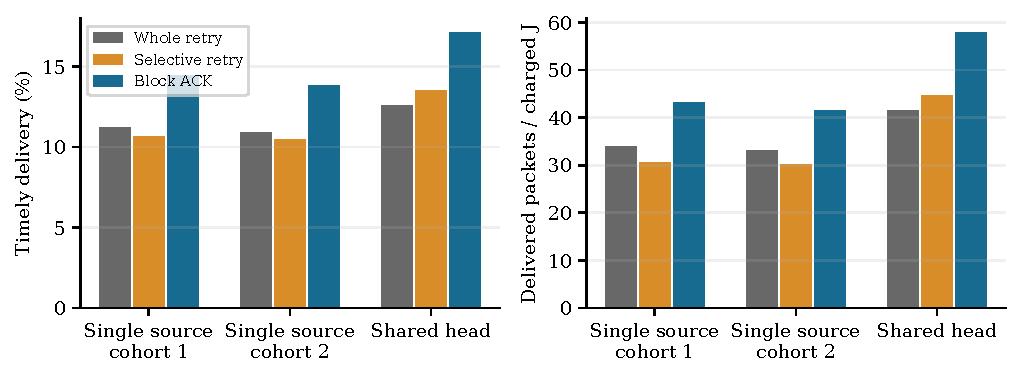
\includegraphics[width=.94\textwidth]{figures/aggregate.pdf}
\caption{Absolute delivery and energy efficiency. Each group is a separate study, with common policy inputs within that group. Physical parameters differ between single-source and shared-head studies; differences across groups are not algorithmic gains.}
\label{fig:aggregate}
\end{figure*}

\subsection{Shared-Head Integration}
Shared-head block ACK improves both endpoints in Table~\ref{tab:aggregate} under common report costs, background expenditure, and relay constraints.

Relative to whole retry, the delivery gain is 36.340\%, with descriptive 95\% interval [33.499\%,39.197\%]. The packets/J gain is 39.611\%, with interval [36.695\%,42.565\%]. Relative to selective retry, the gains are 26.892\% [25.463\%,28.367\%] and 29.822\% [28.319\%,31.379\%], respectively. All adjusted lower bounds remain above the prespecified margin. Figure~\ref{fig:effects} places these gains beside the failed variants.

The absolute delivery increase over whole retry is approximately 4.56 percentage points, not 36.34 percentage points. This distinction matters because relative gains can appear large at a low-delivery operating point. The results indicate an improvement in usable service under the tested constraints, rather than high-reliability operation for an application requiring nearly complete reporting.

\begin{table}[t]
\caption{Primary block-ACK comparisons: relative gains and adjusted lower bounds, in percent}
\label{tab:bounds}\centering\small
\begin{tabular}{llrrrr}\toprule
Study & Base & $\delta_D$ & Lower & $\delta_\eta$ & Lower\\\midrule
Cohort 1 & Whole & 29.226 & 23.529 & 27.847 & 22.319\\
Cohort 1 & Selective & 35.536 & 31.812 & 41.537 & 37.687\\
Shared & Whole & 36.340 & 33.079 & 39.611 & 36.289\\
Shared & Selective & 26.892 & 25.247 & 29.822 & 28.066\\\bottomrule
\end{tabular}
\end{table}

\begin{figure}[t]
\centering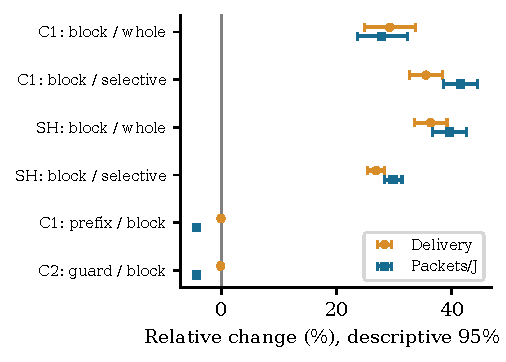
\includegraphics[width=\columnwidth]{figures/effects.pdf}
\caption{Paired relative effects. C1 and C2 denote the single-source cohorts; SH denotes shared head. Bars are descriptive 95\% intervals. The decisions use the more conservative adjusted lower bounds rather than these plotted intervals.}
\label{fig:effects}
\end{figure}

\subsection{Paired Statistical Results}
Table~\ref{tab:paired} reports supplementary paired effects. Shared-head block ACK improves both endpoints against both baselines in all 32 seeds. Adjusted $t$-test values are at most $2.59\times10^{-25}$; adjusted sign-test values are $3.73\times10^{-9}$ for each comparison. The large $d_z$ values reflect consistent differences after averaging 96 scenarios within each seed; they are not packet-level or deployment-level effect sizes.

Neither prefix nor guard significantly changes mean seed delivery relative to block ACK ($p_H=1$). Both reduce packets/J ($p_H<3\times10^{-34}$); every seed has lower efficiency. Failure to reject a delivery difference is not equivalence. Full seed means, sample deviations, raw and adjusted $p$ values, ties, input hashes, and all 22 comparisons accompany the source package.

\begin{table*}[t]
\caption{Supplementary paired-seed effects: candidate minus baseline, pointwise 95\% $t$ intervals, and Holm-adjusted $p_H$ across 22 tests. D: delivery percentage points; E: packets/J.}
\label{tab:paired}\centering\small
\begin{tabular}{lllrrrr}\toprule
Study / comparison & Endpoint & $n$ & Mean difference [95\% CI] & $t$ & $d_z$ & $p_H$\\\midrule
Shared: block--whole & D & 32 & 4.566 [4.299, 4.833] & 34.85 & 6.16 & $2.58\times10^{-25}$\\
 & E & 32 & 16.390 [15.456, 17.323] & 35.81 & 6.33 & $1.22\times10^{-25}$\\
Shared: block--selective & D & 32 & 3.649 [3.444, 3.855] & 36.29 & 6.42 & $8.68\times10^{-26}$\\
 & E & 32 & 13.279 [12.610, 13.948] & 40.50 & 7.16 & $3.32\times10^{-27}$\\
Cohort 1: prefix--block & D & 64 & $-0.014$ [$-0.059$, 0.031] & $-0.62$ & $-0.08$ & 1.000\\
 & E & 64 & $-1.829$ [$-1.943$, $-1.715$] & $-32.01$ & $-4.00$ & $2.42\times10^{-39}$\\
Cohort 2: guard--block & D & 64 & $-0.0001$ [$-0.033$, 0.033] & $-0.01$ & $-0.001$ & 1.000\\
 & E & 64 & $-1.778$ [$-1.913$, $-1.643$] & $-26.30$ & $-3.29$ & $2.26\times10^{-34}$\\\bottomrule
\end{tabular}
\end{table*}

\subsection{Why the Two Extensions Do Not Improve the Comparator}
The affordable-prefix rule produces nearly the same delivery as block acknowledgement in cohort 1: 14.450\% versus 14.458\%. Its packets/J falls to 41.4350 from 43.2781. Relative delivery changes by $-0.054\%$ and efficiency by $-4.259\%$. The corresponding adjusted lower bounds are negative, so the extension fails the declared dual-endpoint requirement.

The completion guard likewise fails on the fresh second cohort. Relative to block acknowledgement, delivery changes by $-0.085\%$ and efficiency by $-4.281\%$. Relative to the prefix policy it changes delivery by $-0.056\%$ and efficiency by $-0.046\%$. The guard therefore cannot be selected by pointing to its comparisons against weaker baselines.

Additional partial windows pay grants, receipts, and the fixed radio envelope without necessarily completing a datagram. Nearly unchanged delivery with greater charged energy supports this explanation, although it is not a complete causal decomposition. The guard may also abstain under pessimistic received state after ACK loss. No threshold is retuned on these cohorts.

\begin{figure*}[!t]
\centering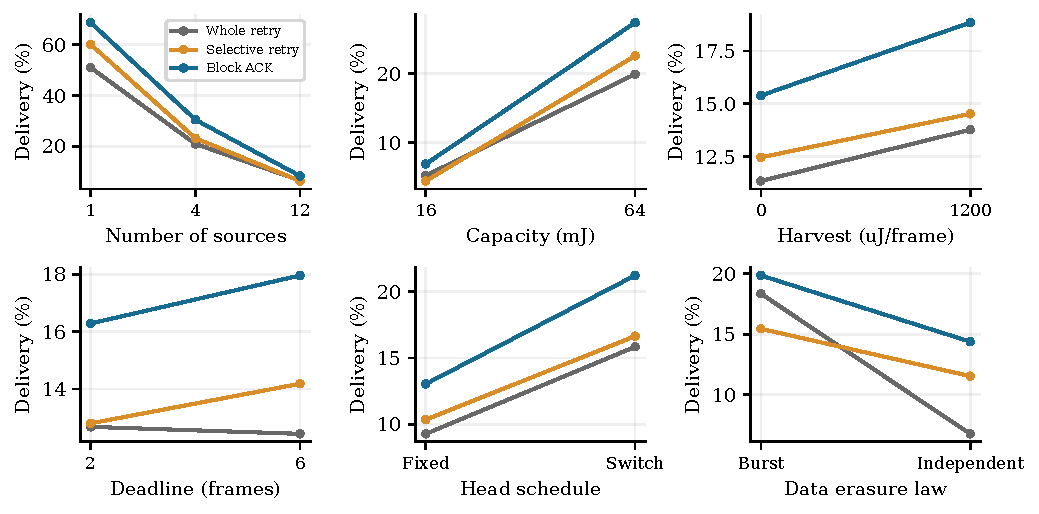
\includegraphics[width=.84\textwidth]{figures/factors.pdf}
\caption{Descriptive shared-head sensitivity. Each point pools all remaining configured factors and paired seeds. Lines guide the eye across discrete settings; they are not interpolated simulation results. All scenario cells remain in the primary analysis.}
\label{fig:factors}

\centering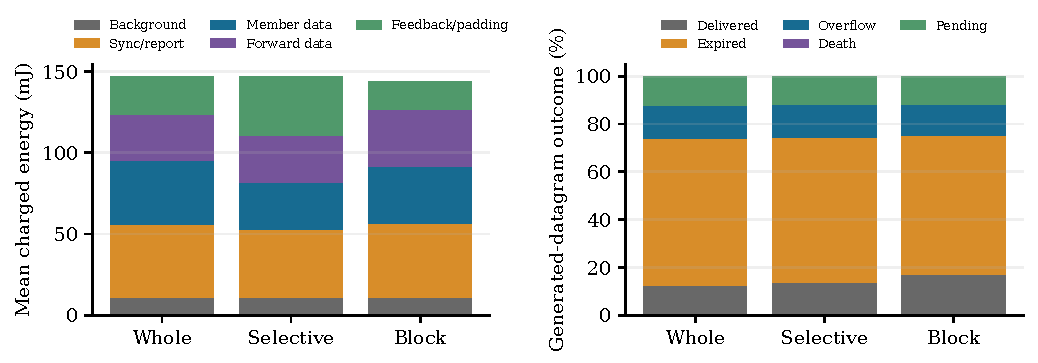
\includegraphics[width=.84\textwidth]{figures/accounting.pdf}
\caption{Shared-head accounting. Left: actual charged energy decomposed into mutually exclusive categories; feedback includes reserved padding and processing residuals. Right: the complete partition of generated datagrams. A delivered packet retained for receipt recovery is counted only as delivered.}
\label{fig:accounting}
\end{figure*}

\subsection{Resource and Source-Count Sensitivity}
Figure~\ref{fig:factors} reports exploratory marginal estimates, averaging other factors; these are not separate superiority tests.

Block delivery falls from 68.739\% at one source to 30.477\% at four and 8.286\% at twelve. One head battery and two live buffers remain fixed: this is resource-sharing stress, not constant-reliability scale-out.

Increasing capacity from 16 to 64~mJ raises block delivery from 6.907\% to 27.335\%; adding harvest raises it from 15.393\% to 18.849\%. Longer deadlines raise delivery from 16.285\% to 17.958\%, while also prolonging buffer occupancy.

Switching heads raises delivery from 13.038\% to 21.205\%, but combines disrupted knowledge with access to a less-used battery. It cannot identify a mobility benefit without a separate matched intervention.

Block delivery is 19.859\% under burst loss and 14.384\% under independent loss. Burst successes can complete a hop block, whereas independent errors disperse missing fragments. Equal marginal success rates therefore need not produce equal recovery workloads.



\subsection{Energy Use and Undelivered Traffic}
Figure~\ref{fig:accounting} reports the energy and packet ledgers rather than only their ratios. For block acknowledgement in the shared study, mean charged energy is 143.669~mJ per episode. Background accounts for 11.040~mJ, sync/report control for 45.270~mJ, member data for 35.057~mJ, forwarded data for 35.518~mJ, and feedback/padding for 16.784~mJ. Control expenditure is therefore material even before recovery feedback is considered.

The same aggregate generates 48.5625 datagrams and delivers 8.3145. Approximately 28.1240 expire, 6.3695 overflow, 5.7529 remain pending and undelivered, and 0.0016 are assigned to source death. Expiry is the largest undelivered category. Absorbing death is uncommon in this aggregate because the admission rule protects future background energy; poor delivery can therefore coexist with many surviving nodes. Survival alone would not describe the service quality of this model.

Block ACK records 7.3506 buffer and 0.0114 airtime rejections per episode. These repeated event counts are not disjoint packet-loss causes. Buffer concentration warrants investigation, but increasing buffers alone need not overcome energy and deadline limits.



\subsection{Implications for Clustered IoT Design}
Recovery, observation, and settlement must be evaluated together. Fewer ACKs change both cost and knowledge; partial service need not complete before its deadline. A deployment must preserve identities, announce transaction boundaries, retain custody, and jointly reserve source and head costs. Buffer admission belongs in that decision because partial reception creates a state obligation. Platform measurements are needed to calibrate guards, radio transitions, and metadata overhead.

\subsection{Interpretation Boundaries}
The scenario grids deliberately expose energy shortage and finite deadlines over a 24-second horizon. They do not establish sustained energy-neutral operation, application-specific reliability, or a complete mobile network's lifetime. Harvest is a configured constant rather than a measured solar/thermal trace. Heads are prescribed dedicated forwarding nodes, and reliable funded sync/report/grant exchange remains an assumption. Spatial fading, collisions, interference, and asynchronous clock behavior are outside the evaluated model.

Firmware that safely sleeps within a transaction could reduce the conservative envelope, whereas control discovery retries could add cost. Their effect on policy ranking requires matched evaluation. The subgroup summaries are exploratory; full-network attribution and performance requirements remain separate from these component screens. The measurements are not pooled with older HTA-MAC network results.

\section{Conclusion}
Joint source/head funding, fixed windows, received feedback, and receipt-based custody provide a reproducible fragment-recovery model with bounded shared relay resources and exact conservation ledgers.

Block ACK achieves 17.12\% delivery and 57.87 packets/J in the shared grid, exceeding the 1\% adjusted-bootstrap margin against both matched baselines. Supplementary paired tests support consistent seed-level gains. Two finer admission variants fail: affordable partial service need not yield useful completed service.

Relay energy and reassembly concentration remain limiting. Next steps are full exogenous head traces, measured harvesting, control losses, a matched published baseline, and untouched confirmation under common accounting.

\section*{Acknowledgment}
OpenAI Codex assisted with manuscript drafting, LaTeX preparation, and figure-generation code.

\begin{thebibliography}{15}
\bibitem{iannello} F. Iannello, O. Simeone, and U. Spagnolini, ``Medium access control protocols for wireless sensor networks with energy harvesting,'' \emph{IEEE Trans. Commun.}, vol. 60, no. 5, pp. 1381--1389, 2012, doi: 10.1109/TCOMM.2012.030712.110089.
\bibitem{rfc4944} G. Montenegro, N. Kushalnagar, J. Hui, and D. Culler, ``Transmission of IPv6 packets over IEEE 802.15.4 networks,'' RFC 4944, Sep. 2007, doi: 10.17487/RFC4944.
\bibitem{rfc8930} T. Watteyne, P. Thubert, and C. Bormann, ``On forwarding 6LoWPAN fragments over a multi-hop IPv6 network,'' RFC 8930, Nov. 2020, doi: 10.17487/RFC8930.
\bibitem{rfc8931} P. Thubert, Ed., ``IPv6 over low-power wireless personal area network (6LoWPAN) selective fragment recovery,'' RFC 8931, Nov. 2020, doi: 10.17487/RFC8931.
\bibitem{rimac} Y. Sun, O. Gurewitz, and D. B. Johnson, ``RI-MAC: A receiver-initiated asynchronous duty cycle MAC protocol for dynamic traffic loads in wireless sensor networks,'' in \emph{Proc. ACM SenSys}, 2008, pp. 1--14, doi: 10.1145/1460412.1460414.
\bibitem{rfc7554} T. Watteyne, M. R. Palattella, and L. A. Grieco, ``Using IEEE 802.15.4e time-slotted channel hopping (TSCH) in the Internet of Things (IoT): Problem statement,'' RFC 7554, May 2015, doi: 10.17487/RFC7554.
\bibitem{rfc8180} X. Vilajosana, K. Pister, and T. Watteyne, ``Minimal IPv6 over the TSCH mode of IEEE 802.15.4e (6TiSCH) configuration,'' RFC 8180, May 2017, doi: 10.17487/RFC8180.
\bibitem{scanzio} S. Scanzio, G. Formis, T. Facchinetti, G. Paolini, and G. Cena, ``Wireless sensor networks based on TSCH/TDMA with power consumption and latency constraints,'' arXiv:2411.12879, 2024.
\bibitem{vanleemput} D. Van Leemput, J. Famaey, J. Hoebeke, and E. De Poorter, ``Energy-aware adaptive scheduling for battery-less 6TiSCH routers in industrial wireless sensor networks,'' \emph{IEEE Access}, vol. 12, pp. 180034--180047, 2024, doi: 10.1109/ACCESS.2024.3508540.
\bibitem{rlasl} F. F. Jurado-Lasso and J. F. Jurado, ``RL-ASL: A dynamic listening optimization for TSCH networks using reinforcement learning,'' arXiv:2604.07533, 2026.
\bibitem{heart} ``HEART-CH: Hybrid-energy-aware spatiotemporal reinforcement learning for cluster-head selection in mobile IoT sensor networks,'' unpublished manuscript, supplied copy, Sep. 2026.
\bibitem{cc2420} Texas Instruments, ``CC2420: 2.4 GHz IEEE 802.15.4 / ZigBee-ready RF transceiver,'' device specifications. [Online]. Available: \url{https://www.ti.com/product/CC2420}. Accessed: Sep. 24, 2026.
\bibitem{efron} B. Efron, ``Bootstrap methods: Another look at the jackknife,'' \emph{Ann. Statist.}, vol. 7, no. 1, pp. 1--26, 1979, doi: 10.1214/aos/1176344552.
\bibitem{holm} S. Holm, ``A simple sequentially rejective multiple test procedure,'' \emph{Scand. J. Statist.}, vol. 6, no. 2, pp. 65--70, 1979.
\bibitem{artifact} ``HTA-MAC fragment-repair evidence release,'' source and simulation artifacts, commit 0e12c49, Sep. 21, 2026. [Online]. Available: \url{https://github.com/thomvs-dev/hta-mac-ehwsn/tree/0e12c49b9f554cb0eb22a1d84cd531eb61ed8508/evidence/fragment_repair_20260921}.
\end{thebibliography}
\end{document}
